%%%% fabiundstefan.tex
%%%%
%%%% Technical report for the Travel Planning Challenge @ IJCAI 2026.
%%%% VERSION 3 DRAFT (2026-08-07). Supersedes v2 and incorporates every annotation in
%%%% report/feedback/fabiundstefan_v2.pdf; see report/README.md for the resolution map.
%%%%
%%%% Requirements: official IJCAI template, max 4 pages, not double-blind, PDF named after the team.
%%%% Build: cd report && make
%%%% Figures: .venv/bin/python scripts/report_figures.py
%%%%
%%%% Every numerical claim traces to a committed artifact named in a nearby comment:
%%%%   ROW    = results/phase2_baselines/full_runs/<id>.json
%%%%   SCREEN = results/phase2_baselines/screens/<name>/
%%%%   PORTAL = organizers' returned result

\documentclass{article}
\pdfpagewidth=8.5in
\pdfpageheight=11in

\usepackage{ijcai26}
\usepackage{times}
\usepackage{url}
\usepackage[hidelinks]{hyperref}
\usepackage[utf8]{inputenc}
\usepackage[small]{caption}
\usepackage{graphicx}
\usepackage{amsmath}
\usepackage{amsthm}
\usepackage{booktabs}

\urlstyle{same}
\setlength{\textfloatsep}{10pt plus 2pt minus 2pt}
\setlength{\floatsep}{10pt plus 2pt minus 2pt}
\setlength{\intextsep}{10pt plus 2pt minus 2pt}

\pdfinfo{
/TemplateVersion (IJCAI.2026.0)
}

\makeatletter
\newcommand\footnoteref[1]{\protected@xdef\@thefnmark{\ref{#1}}\@footnotemark}
\makeatother

\title{Agentic Travel Planning:\\Where AI Helped, and Where It Did Not}

\author{
\begin{tabular}{c@{\hspace{2.4cm}}c}
Stefan Schneider & Fabian Missbrenner\\[-0.1em]
\textnormal{\normalsize\texttt{stefanbschneider@outlook.com}} &
% \textnormal{\normalsize Technische Universit\"at Berlin}\\[-0.1em]
\textnormal{\normalsize\texttt{mail@fabimi.net}}
\end{tabular}
}

\begin{document}

\maketitle

\begin{abstract}
Many agentic tasks begin with an open-ended goal but are useful only when hard
constraints are met. Multi-day travel planning is a popular example for such a task. 
We describe our entry to the ``2nd Travel Planning Challenge with Agentic AI'' at the IJCAI 2026 conference\footnote{\label{tpc}Website: \url{https://chinatravel-competition.github.io/IJCAI2026/}, Benchmark: \url{https://github.com/LAMDA-NeSy/ChinaTravel} (URLs accessed on August 9, 2026)}.
Curiously, we found that the best-performing system was a deterministic, environment-grounded
planner that completely ignores the available large language model~(LLM).
Instead, it uses classical optimization and acceptance gates that can only emit itineraries confirmed valid
against the environment rules and APIs. 

Conversely, AI agents were most valuable in building and improving that system:
We successfully used the competition as a low-risk environment to run a near-continuous data-driven multi-agent AI development process, 
generating hundreds of commits over eight weeks. 
The agents proposed experiments, implemented changes, ran evaluations, and reviewed pull requests, while humans made every decision that mattered: 
what to prioritize and how to split the work, how to measure progress and provide a fast, meaningful feedback loop for the agents, and what to finally submit.
% The first official held-out submission sharpened this division of labor: grounding
% generalized, while constraint extraction tuned to one phrasing style did not.
% Repairing that gap is what the second version contains: on unfamiliar phrasing it
% raises the clause satisfaction rate from 75.6 to 92.3 and the share of fully
% satisfied itineraries from 10.7\% to 65.3\%. We also report how the system was
% built --- near-continuous multi-agent ``vibe coding'' behind a deterministic
% evaluation harness --- as a result in its own right.
\end{abstract}

\section{Introduction}
\label{sec:intro}

Many real-world tasks involve a loosely stated human goal that needs to be turned
into an output that is not merely plausible but correct. For example, multi-day travel
planning combines fuzzy human requirements that must be turned into exact
constraints for the constructed itinerary to fulfill.
The IJCAI 2026 Travel Planning Challenge\footnoteref{tpc}
extends the ChinaTravel benchmark of Shao et al.~\cite{shao2024chinatravel}: for a given human travel intent, an agent must
produce a preference-aligned itinerary between a selection of Chinese cities. A request
might say:
\begin{quote}
\small ``Plan three days in Suzhou, visit the Humble Administrator's Garden
between 9 and 11, stay near the old town, avoid taxis, and spend at most CNY 3,000.''
\end{quote}
The output is structured data, not free text. Hotels, attractions, and restaurants
must exist in the provided sandbox environment; opening hours, transportation, and costs must be
consistent; logical requirements must hold; and commonsense rules such as meal
counts must pass. The evaluator measures environmental validity (EPR), logical
satisfaction (C-LPR and FPR), and preferences. Hard constraint satisfaction heavily dominates the overall score -- preference terms only count if all hard requirements are fulfilled (else set to zero).

The competition has two phases. In the offline first phase, released verifier
fields and a generous time budget allowed us to satisfy almost all constraints
and then polish preferences. In the harder phase 2, which we focus on in this report, only
query text and environment tools are exposed to the agent. 
For each query, the agent must infer what constraints to satisfy and how -- within 5~hours total for 100 unknown queries.

Our system follows a propose--verify--repair pattern related to LLM-Modulo
systems~\cite{kambhampati2024llmmodulo}, but assigns roles asymmetrically:
an optional LLM may interpret language or propose changes; environment APIs
establish facts; and deterministic optimization and checks decide what may be
emitted. Our final configuration disables the LLM path.

\section{System Design}
\label{sec:system}

\subsection{Pipeline and trust boundary}

Figure~\ref{fig:architecture} follows the example from language to a simplified
itinerary. Oracle verifier fields are removed before execution (only available in the public data, not the held-out test set). The only inputs
are visible query text and allowed environment tools. Every point of interest~(POI), hotel,
restaurant, price, opening hour, and transportation record is read from
\texttt{WorldEnv}; nothing is generated as a plausible substitute.

\begin{figure*}[t]
\centering
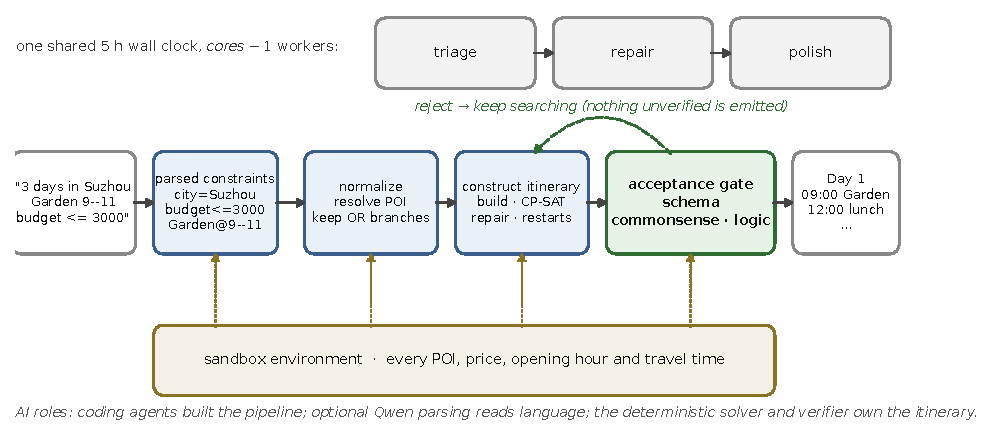
\includegraphics[width=0.90\textwidth]{figures/architecture.pdf}
\caption{The per-query pipeline and whole-run scheduler, illustrated with the
opening example. Optional model-based extraction may fill missing constraints;
grounding, construction, repair, and acceptance remain deterministic.}
\label{fig:architecture}
\end{figure*}

\subsection{Parsing and normalization}

The parser extracts dates, cities, budgets, excluded transportation, named POIs,
timed visits, hotel properties, room counts, cuisines, and attraction categories.
It also handles alternatives (``visit A \textit{or} B'') by creating separate solver variants rather than an impossible conjunction. Grounding
and normalization resolve names and concepts against each city's catalog.
Deterministic extraction is fast and testable but not synonymous with
understanding, so we added phrasing-robust fallbacks for the largest measured
recall gaps and an optional LLM\footnote{The organizers provide a Qwen3.6-27B model for evaluation.} extractor that may fill a missing family but never
overwrite a deterministic value. Section~\ref{sec:ai} compares this path with
the deterministic extractor and explains why it is disabled in our final agent.

Precision is equally important. Our audit found that in 23--50\% of free-prose
queries, depending on the set, the parser initially invented a required POI name that did
not exist in the target city.
% SCREEN: results/phase2_baselines/screens/20260807_p22_unsatisfiable_names/README.md
Such a query has no feasible solution at all, so it can never earn a full-plan
point no matter how long the solver runs. Therefore, a catalog check in the final parser removes such
provably unsatisfiable required names and category values, after first trying to
salvage a real POI name from the captured text. It reduced this measured failure
class to zero on every set we hold.
% SCREEN: results/phase2_baselines/screens/20260808_p22_salvage_before_drop/README.md

Further investigation illustrates how narrow these parsing gaps are. Until a recent fix to our final agent, intercity
transport was the largest remaining unextracted family on the free-prose dataset: the
extractor recognized ``take the train to the destination'' but not ``we have
chosen to fly'' or ``by high-speed train (G)'', missing 33 of 85 such
requirements on one released set and 27 of 32 on another. Adding verb-form and
qualified-noun patterns, guarded so that a station name or an undecided
``fly or take the train'' never produces a requirement, removed most of them
while leaving precision and the familiar register unchanged.
% SCREEN: results/phase2_baselines/screens/20260808_v2_candidate_freeprose/README.md

\subsection{Construction, repair, and densification}

The deterministic planner constructs a complete base itinerary from grounded
candidate pools. It then applies bounded CP-SAT~\cite{ortools},
domain-specific repairs, and seeded restarts. Repairs include placing named
activities inside requested windows, inserting absent required POIs, closing
transportation gaps, and rebuilding intercity legs. The same acceptance checker
evaluates every candidate: query constraints, schema, and commonsense rules must
all pass. Accepted candidates are ranked by preference value and cost.

Packing and densification add meals and activities only while the checker keeps
passing. A minimal schema-valid itinerary is written before solving so an
interrupted run still has output --- availability, not success, since an empty
itinerary scores zero.

\subsection{Scheduling the five-hour run}

The whole-split scheduler uses \emph{triage}, \emph{repair}, and \emph{polish}
passes in parallel across queries: triage reaches every query cheaply, repair
revisits the nearest failures with larger budgets, and polish spends what is left
only after hard requirements pass. A keep-best rule makes updates monotonic, and
deadline checks prevent starting work that cannot finish. As summarized in
Figure~\ref{fig:architecture}, triage quickly constructs an accepted candidate
for every query; repair re-solves near misses with increasing per-query budgets;
and polish optimizes preferences for passing plans. Each accepted improvement is
written immediately, so a limited budget or interrupt leaves the best plan found.

\section{Evaluation}
\label{sec:evaluation}

We evaluate three questions: what official feedback says about generalization,
what changed fro our v1 to v2 submission, and whether deterministic planning outperforms
model-based baselines. We call the released template-style queries
\emph{familiar} and the differently worded extensions to the public ChinaTravel
dataset \emph{free prose}\footnote{\url{https://huggingface.co/datasets/LAMDA-NeSy/ChinaTravel},
explicitly referenced by the organizers.}.

\subsection{Official feedback}

In the final, second phase of the competition, the organizers permit two submitted harness versions and retain the better score.
We submitted v1 early to obtain the only available held-out feedback before
choosing v2. On the held-out set, our overall score was 33.25 versus the leader's 36.41.
% ROW: results/phase2_baselines/full_runs/20260807T152009Z.json
% PORTAL: results/phase2_baselines/heldout/20260807_v1_leaderboard.json
% PORTAL: results/phase2_baselines/heldout/20260808_leaderboard_5teams.json

Grounding generalized: micro EPR---the share of itinerary fields consistent with
the environment---remained 99.48, within 0.16 of the best entry. Constraint
understanding did not: C-LPR---the share of requested clauses satisfied---fell
from 90.08 on familiar queries to 55.20 held out. No query passed every
requirement, so all preference terms were zero.

Across the five submitted systems, four had a full-plan rate of zero and the
fifth had one point; every preference term was zero. Thus full-plan failure was not
unique to us, but our C-LPR drop pointed specifically to parsing and motivated
the v2 extraction work below. The entire 3.16-point gap to the leader corresponds
to 12.6 clause points.
% PORTAL: results/phase2_baselines/heldout/20260808_leaderboard_5teams.json

\subsection{What the second version changes}

In the final two days before the deadline, we repaired the phrasing brittleness
described below, removed
the unsatisfiable-name failure class, and closed the largest remaining recall
gaps. None of that is visible on the familiar register, where the extractor was
already complete, so we measured it where it applies: 150 differently phrased
released queries, both builds run as a paired experiment at identical budget on
one host, scored against an English-literal oracle so the full-plan rate has a
real denominator.\footnote{Those released sets state their query text in English
but their verifier literals in Chinese, which caps the achievable full-plan rate;
we translate the literals with an audited one-to-one map for measurement only,
and the agent never reads them.} Figure~\ref{fig:v1v2} shows the result: the
clause rate rises from 75.6 to 92.3 and the full-plan rate from 10.7 to 65.3.
Checked clause by clause, 225 of 1264 clauses move from failing to passing
against 13 lost, and the number of queries satisfying every requirement rises
from 16 to 98 of 150.
% SCREEN: results/phase2_baselines/screens/20260808_v2_candidate_freeprose/README.md
% SCREEN: results/phase2_baselines/screens/20260809_r34_intercity_e2e/README.md
On the familiar register, where most of this cannot help, a paired run of the
full five-hour pipeline confirms no regression and a modest gain: 64.69 to 66.81
overall, with the full-plan rate moving from 45 to 49 of 100 queries.
% ROW: results/phase2_baselines/full_runs/20260808T200402Z_v2gate_base.json
% ROW: results/phase2_baselines/full_runs/20260808T200402Z_v2gate_cand.json
% ROW: results/phase2_baselines/full_runs/20260809T055547Z_p28gate_cand.json
% SCREEN: results/phase2_baselines/screens/20260809_p28_room_count/README.md

\begin{figure}[t]
\centering
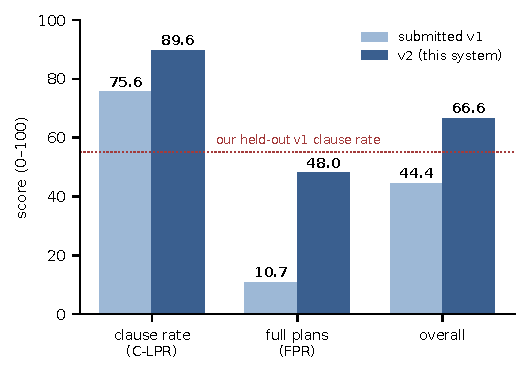
\includegraphics[width=\columnwidth]{figures/v1_v2_free_prose.pdf}
\caption{Submitted v1 versus the second version on 150 unfamiliar-phrasing
queries, paired at equal budget; higher is better. The dotted line is our v1
clause rate on the organizers' held-out set, a different query set, shown for
scale. At the time of writing, our v2 agent is prepared but not submitted, so its held-out
score is unknown.}
\label{fig:v1v2}
\end{figure}

The largest single fix illustrates a measurement lesson. Our coverage audits
classified the hotel room count as ``guaranteed by trip metadata'', because the
planner derives it from party size and beds per room --- correct only when the
traveler says nothing. Asking a different question, \emph{for each query that fails
exactly one requirement, which requirement is it?}, showed that 28 of 150
free-prose queries failed \emph{only} the room count: one field away from
satisfying everything. Reading the stated count instead of deriving it moved the
full-plan rate on that set from 48\% to 65\%. No coverage table could have found
this; a near-miss analysis found it in minutes.
% SCREEN: results/phase2_baselines/screens/20260809_p28_room_count/README.md

% We deliberately do not convert these numbers into a predicted held-out score. It
% is one register, and the last prediction we made from a local number was wrong by
% a factor of two. What they establish is direction and size in the metric that
% currently decides the ranking.

\subsection{Query phrasing}
The familiar released set was presented as in distribution, so prioritizing it was
a reasonable choice. Its queries use a regular numbered template, whereas other
released sets express the same requirements in varied prose: offline audits found
no missed clauses on the familiar register but 12--29\% on the differently phrased
ones. We had optimized against the one register we were already perfect on.
% SCREEN: results/phase2_baselines/screens/20260807_generalization_post_p15/README.md

\subsection{Planning baselines}

We ran two small, matched comparisons. An autonomous tool-using Qwen agent scored
1.88 and 2.64 on eight familiar and eight free-prose queries, versus 67.71 and
48.49 for our solver; the upstream RuleNeSy baseline \cite{shao2024chinatravel}
scored about 9.5 on four of each. Neither produced an itinerary passing every
commonsense rule.
% SCREEN: results/phase2_baselines/screens/20260806_llm_arms/README.md
These samples are too small to rank systems, but the failure modes support
retaining deterministic acceptance and optimization: on these samples our
solver scored 18--36 times higher than autonomous Qwen and about five to seven
times higher than RuleNeSy.

\section{Where AI Helped --- and Where It Did Not}
\label{sec:ai}

\subsection{A safe vibe-coding experiment}

We used this challenge deliberately as a low-risk environment in which to push
agent-driven development (``vibe coding'') much harder than we would on a production system.
With an objective scorer, nothing deployed, and no external dependencies, we
could ask how far coding agents can carry a real system given fast feedback.

Very far, as it turned out, given a great deal of scaffolding and proper initial design. We ran multiple
paid agent subscriptions across several machines, with one or more agents working
almost continuously for eight weeks. The result is hundreds of commits, 100+ reviewed and merged
pull requests, more than 1000 tests, and dozens of long-running evaluation
measurements. Humans still made every
decision that mattered: what to prioritize and
how to split the work, how to measure progress and
provide a fast, meaningful feedback loop for the
agents, and what to finally submit.
Three practices worked well:

\textbf{1. Split repeating work into different agent roles.} Expensive reasoning
models were used for analysis, diagnosis, and planning: reading measurements,
proposing the next experiment, ranking work by expected effect. Faster, cheaper
agents then implemented a specified change with tests, and ran evaluations. The
planning agent maintained a ranked work list; implementation and evaluation
proceeded in parallel branches against it, preventing implementing agents from
silently redefining their task. Cheaper agents could ask a stronger advisor for
guidance.

\textbf{2. Make feedback fast, automatic, and cheap to trust.} We invested more in
the evaluation harness than in any single planner feature: a paired A/B screen
that decides in one or two hours whether a change is worth a long run, a whole-run
mode reproducing the submission's exact shape, deterministic seeds, and result
ledgers recording every condition needed to decide whether two numbers may be
compared. Agents could then evaluate their own work overnight and report a verdict
against a criterion written before the run. We split available data into
validation and held-out sets to limit overfitting.

\textbf{3. Write the invariants down and enforce them by tests.} Grounding,
no oracle leakage, acceptance-before-emission, and evaluation proof before enabling new features are
project rules pinned by tests, so an agent that would violate one fails rather than
persuades. Cold-start verification caught a start-up race that would have shipped
empty itineraries for a whole split while still exiting successfully.

Two limits are worth stating. The volume of agent output is not itself a result:
much of it was superseded, and the ratio of committed work to accepted improvement
was correspondingly low. Agents were also often over-optimistic about their changes,
making rigorous evaluation and promotion essential.

\subsection{Inside the system}

We tested the LLM in three distinct roles: parsing, repair, and end-to-end
planning. For these experiments, we used the DeepInfra API, which provides the same Qwen3.6-27B
model version used by the organizers without a local deployment. LLM-first extraction cut
missing free-prose constraint families by 40--65\%, but initially converted many
misses into values that did not match the environment vocabulary.
% SCREEN: results/phase2_baselines/screens/20260806_llm_arms/README.md
We therefore connected model output to the same city-specific entity and category
catalogs used by the solver. Grounded, fill-only extraction improved one small
familiar A/B test but was flat on the matched free-prose subset, and still matched fewer
clauses than the contemporaneous deterministic parser.
% SCREEN: results/phase2_baselines/screens/20260807_p16_entity_resolution_probe/README.md
Our final agent consequently makes zero LLM calls, while retaining the
grounded extractor as an optional path. This is not a rejection of LLM parsing in general;
it separates recognizing a requirement from resolving its values against the
actual database.

We retain the optional parser because implicit categories that no pattern names
still suit a language model, provided its answer is resolved against the closed
vocabulary.
% SCREEN: results/phase2_baselines/screens/20260809_r35_preference_verb_trigger/README.md

We also tried a hybrid: letting a model repair itineraries the checker
rejected, with every proposed edit re-verified before it could be kept. On ten
deterministic failures the loop iterated, proposed valid-looking edits, and
flipped none of them to passing. That's why we did not enable it in the final system.
% SCREEN: results/phase2_baselines/screens/20260808_r27_llm_repair_loop/README.md

End-to-end itinerary generation was the clearer boundary. Even with environment
tools, autonomous Qwen planning accumulated small inconsistencies, and one
violation invalidated the whole itinerary. Dates, opening windows, travel times,
budgets, meals, and disjunctions remain a constrained optimization problem, where
deterministic solving provides reproducibility, explicit acceptance, and efficient
targeted repair.

\section{Conclusion}
\label{sec:conclusion}

We approached this travel planning challenge by hybrid division of labor: 
coding agents accelerated
construction and analysis, while the final agent itself is deterministic and makes
zero LLM calls. Environment tools supply facts, deterministic search assembles
them, and acceptance gates admit only verified plans. Official v1 feedback showed
that grounding transferred while extraction tuned to familiar phrasing did not;
our v2 submission measurably repairs that gap.

The transferable lesson is methodological: agentic coding works well in an
isolated project with fast, objective feedback. Written invariants, comparable
measurements, and independent promotion runs mattered more than output volume.
Models may help at the grounded language--symbol boundary, but our measured model
path did not beat deterministic extraction, and classical optimization remained
better for itinerary construction.

If we wanted to extend our travel planning agent to become a production system, we would replace the sandbox environment with live map, hotel, rail, flight,
and booking APIs, and would infer user-specific objectives rather than inherit
fixed challenge preferences: some travelers want four attractions per day, others
value unplanned time. Live availability would require replanning, but the same
division holds: AI interprets intent, APIs establish reality, optimization
constructs the itinerary, and deterministic verification decides what to emit.

\paragraph{Acknowledgments.}
We thank the organizers for the challenge, benchmark tooling, and clarifications.
{\footnotesize
\bibliographystyle{named}
\bibliography{ijcai26}
}

\end{document}
